%! Author = oli
%! Date = 12/24/23

% Preamble
%\documentclass[10pt,twocolumn,letterpaper]{article}
\documentclass[10pt]{article}

\usepackage{color}

% Packages
\usepackage{amsmath}
\usepackage{chemfig}
\usepackage[utf8]{inputenc}
\usepackage{acronym}
\usepackage{hyperref}
\usepackage{subfig}
\usepackage{graphicx}
\usepackage{float}
\usepackage{tikz}
\usepackage{subcaption}
\usepackage{amssymb}
\usepackage{eurosym}
\usepackage{subcaption}

\title{Filamente und mehr}
\author{Oliver Schütz}

\begin{document}

    \maketitle

    \begin{abstract}
        \textit
        {Der 3D-Druck ist ein Herstellungsverfahren, das es erlaubt, aus verschiedensten Materialien jegliche Formen herzustellen.
        Mit herkömmlichen Verfahren ist dies nicht möglich.
        Jedoch braucht es dafür spezielle Materialien, die entsprechende Eigenschaften aufweisen.
        Hier beschränken wir uns auf Materialien, die mit dem FDM-Verfahren verarbeitet werden können, genauer gesagt auf Filamente.}
        FDM steht für Fused Deposition Modeling, was auf Deutsch etwa Schmelzschichtung bedeutet und ist das am weitesten verbreitete 3D-Druckverfahren.
        Dabei wird ein Kunststoffdraht, das sogenannte Filament, durch eine Düse gepresst und auf einer Druckplatte Schicht für Schicht aufgetragen, woraus das Druckobjekt entsteht.
    \end{abstract}


    \section{Materialien}
    Es gibt verschiedene Arten von Materialien, die sich in Farbe, Form und Material unterscheiden.

    \subsection{Farben und Formen}
    Bei dem FDM-Druck kann grundsätzlich mit allen Farben und Formen gedruckt werden.
    Die verbreitetste Art ist das Filament.
    Zu Beginn der Produktion liegt das Material roh und farblos vor, z.B. als Granulat oder Pellets.
    Obwohl es üblich ist die Pellets zu Filamenten zu verarbeiten, ist es auch möglich, direkt mit den Pellets zu drucken (Pellet-Extruder).


    \begin{figure}[H]
        \centering
        \subfloat[\centering PLA]{{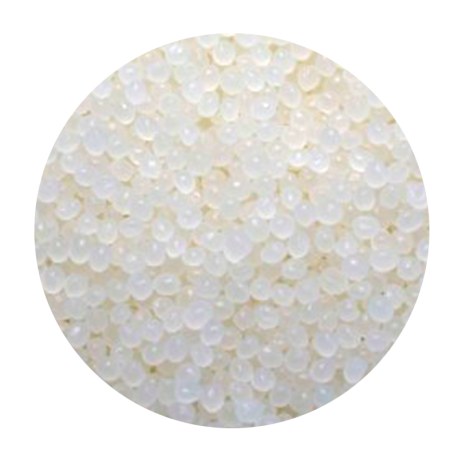
\includegraphics[width=5cm]{img/PLA-Pellets}}}%
        \qquad
        \subfloat[\centering PETG]{{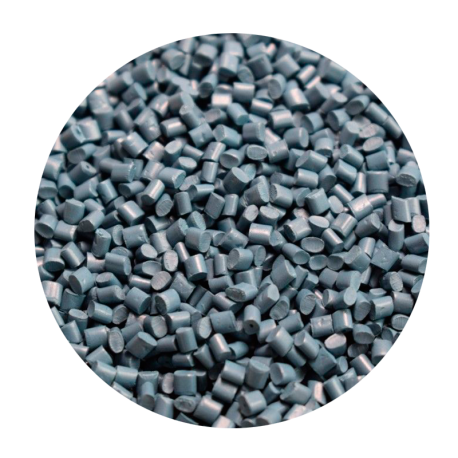
\includegraphics[width=5cm]{img/PETG-Pellets}}}%
        \caption*{Beispiel für Pellets oder Granulat als Ausgangsmaterial für Filamente}
    \end{figure}

    \subsection{Filamentherstellung}
    Im ersten Schritt vermischt man die Pellets mit Farbstoffen oder anderen Materialien, um die gewünschte Farbe zu erhalten oder die Eigenschaften des Materials zu verändern.
    Beispiele für das Beimischen von anderen Materialien sind Kohlefasern, um das Filament stabiler zu machen, TPU um es flexibler zu machen oder Holzfasern, um es wie Holz aussehen zu lassen.
    Bei teureren Filamenten wird das Gemisch anschließend noch getrocknet, um die Feuchtigkeit zu entfernen.
    Macht man dies nicht, kann es zu Blasenbildung im Filament kommen, was zu schlechteren Druckergebnissen führt.

    \begin{figure}[H]
        \centering
        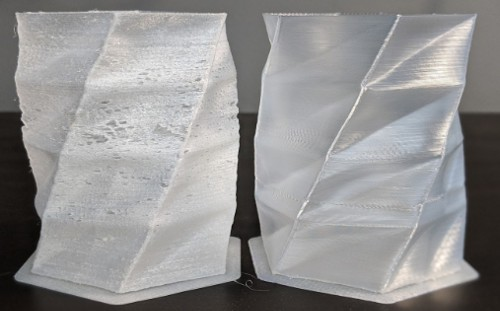
\includegraphics[width=10cm]{img/wet_filament}
        % Zwei captions nebeneinander
        \caption*{Links: Filament mit Feuchtigkeit; Rechts: Getrocknetes Filament}
    \end{figure}



    Anschließend wird das Gemisch in einem Extruder zu Filament verarbeitet.
    Durch einen Trichter gelangt das Granulat / Pellets in eine Extrusionseinheit.
    Dort wird es durch eine Schnecke gefördert und durch gleichzeitiges Erhitzen in einen zähen Kunststoffzustand überführt.
    Am Ende der Schnecke wird das Material durch eine Düse gepresst, die den Durchmesser des Filaments bestimmt und es in die gewünschte Form bringt.

    \begin{figure}[H]
        \centering
        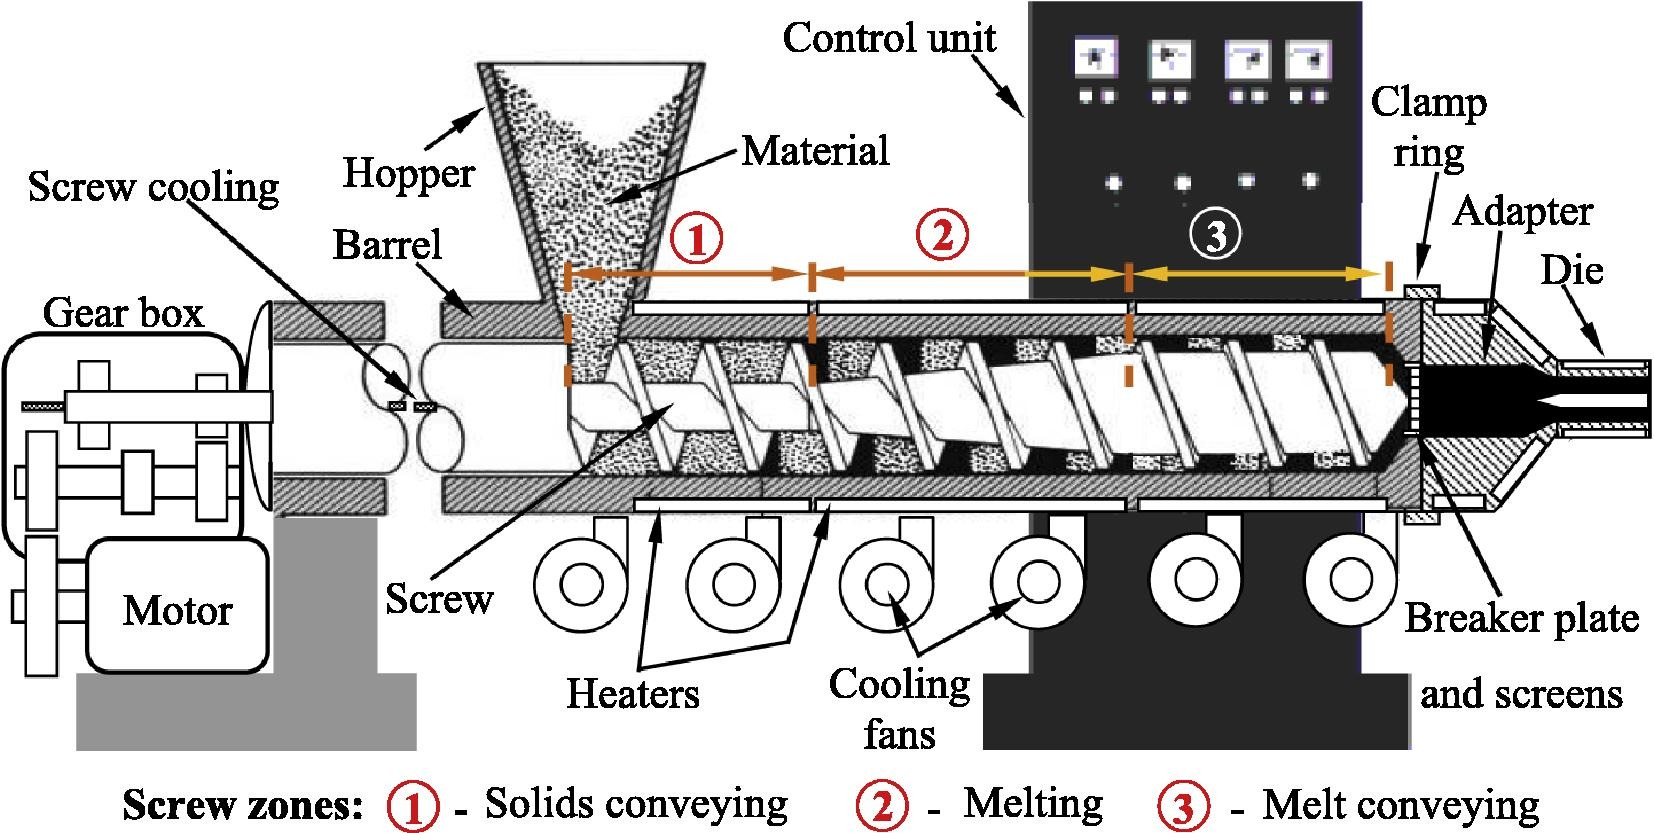
\includegraphics[width=10cm]{img/Production}
        \caption*{Extruder}
    \end{figure}

    Da das Filament nach dem Extrudieren noch heiß und sehr weich ist, würde es sich von selbst verformen.
    Deshalb wird der Filamentstrang durch eine Kühlvorrichtung geführt, das ihn stabilisiert und abkühlt.


    \begin{figure}[H]
        \centering
        \subfloat[\centering Extruder]{{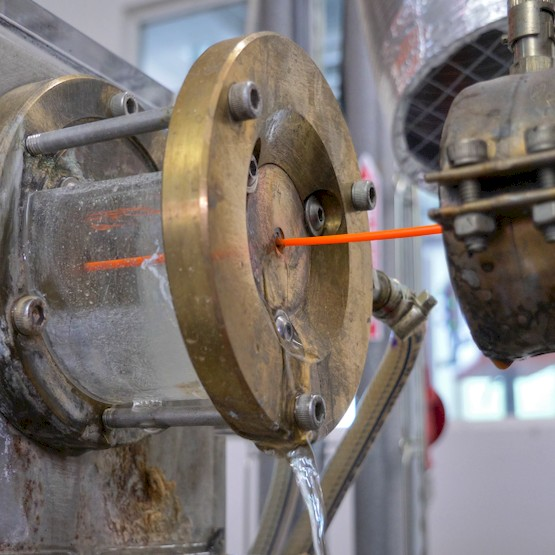
\includegraphics[width=5cm]{img/Extruder}}}%
        \qquad
        \subfloat[\centering Kühlbecken]{{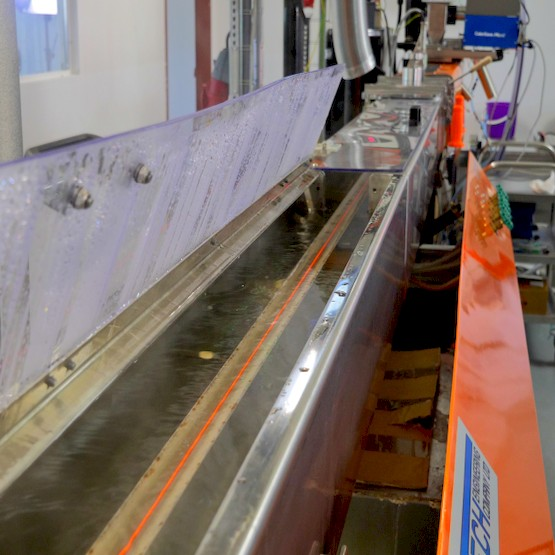
\includegraphics[width=5cm]{img/Kuehler}}}%
    \end{figure}

    \newpage
    Abschließend wird das Filament noch auf Toleranz des Durchmessers geprüft und auf die Spulen gewickelt.

    \begin{figure}[H]
        \centering
        \subfloat[\centering Toleranzmessung]{{\includegraphics[width=5cm]{img/Qualität}}}%
        \qquad
        \subfloat[\centering Wickelung]{{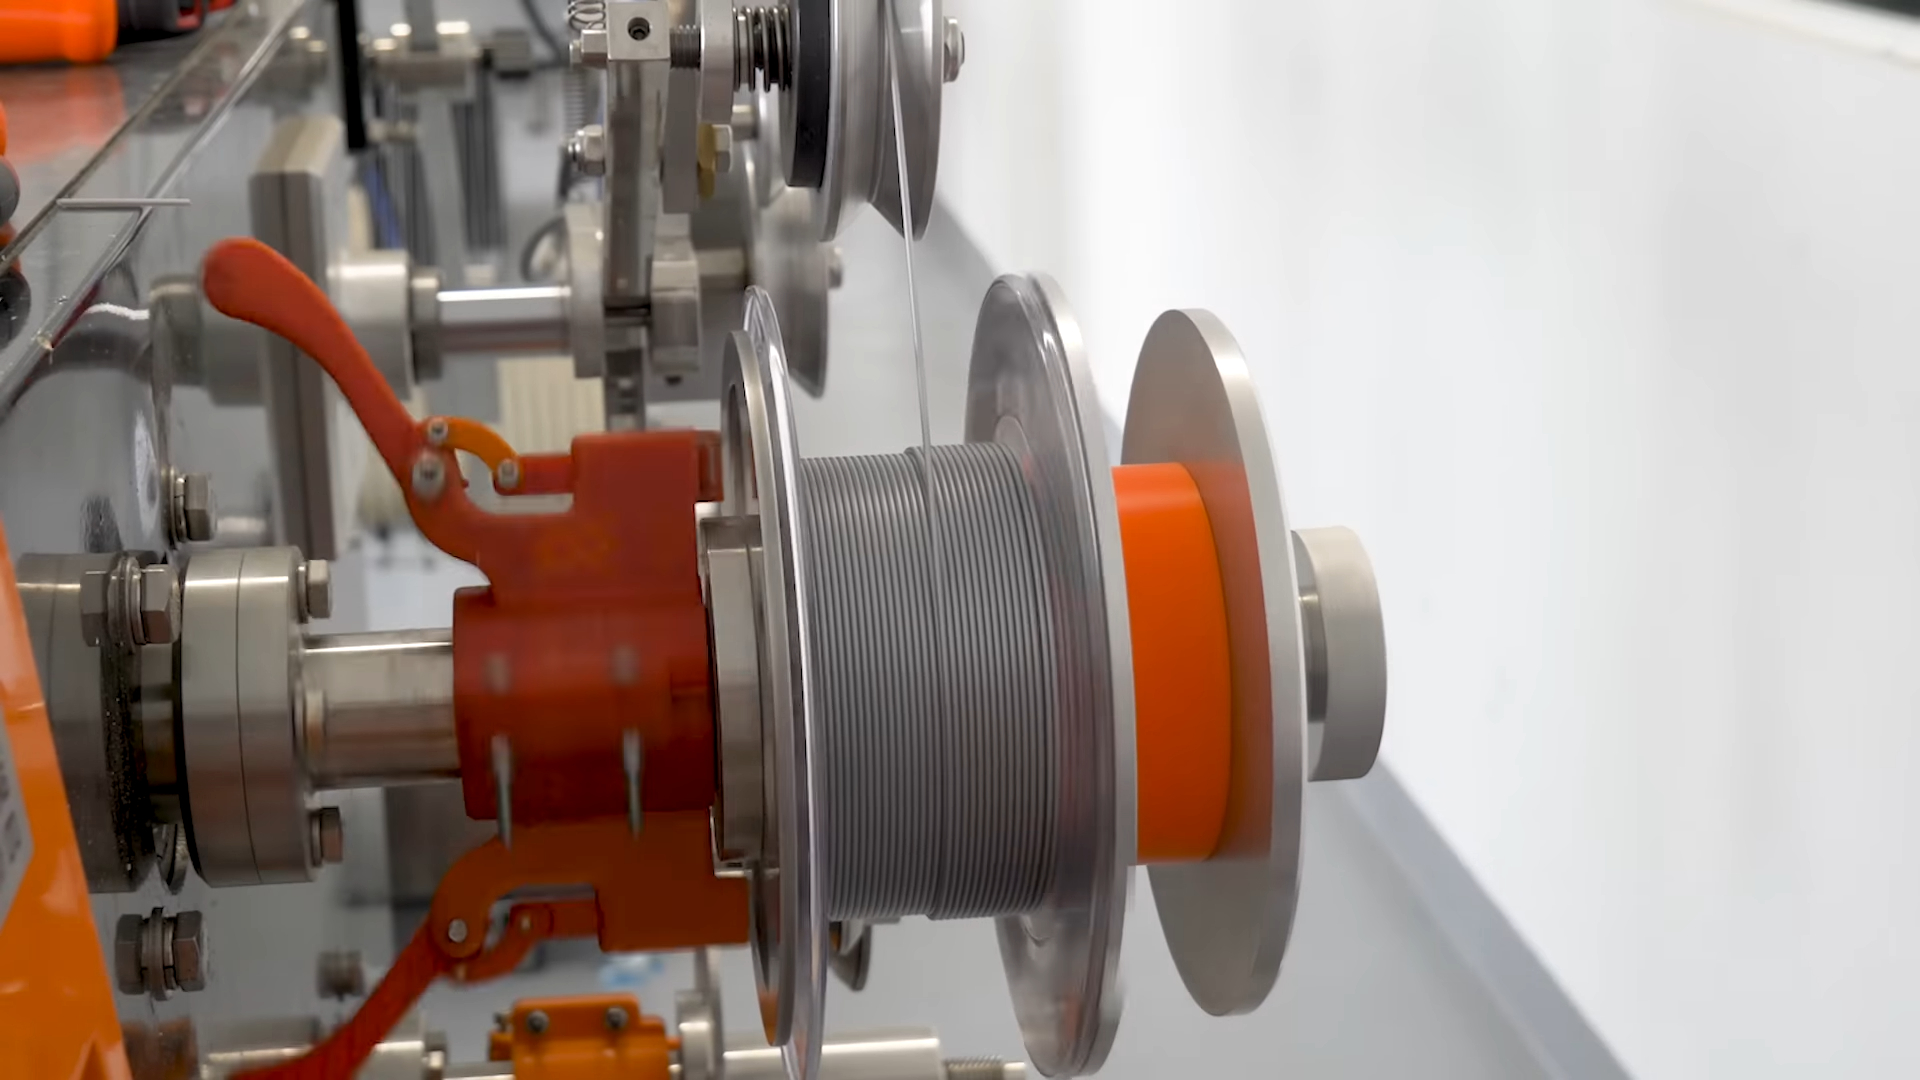
\includegraphics[width=5cm]{img/Wickellung}}}%
    \end{figure}


    \subsection{Recycling}
    Wie bei fast allen Herstellungsverfahren, entsteht auch beim 3D-Druck Abfall.
    Das Filament kann jedoch wieder eingeschmolzen und zu neuen Filamenten verarbeitet werden.
    Dazu wird das Filament geschreddert und zu Granulat verarbeitet.
    Anschließend kann es wieder als Ausgangsmaterial für die Filament Herstellung verwendet werden.
    Zudem lassen sich auch weitere Kunststoffprodukte wie PET-Flaschen oder Spritzgussteile recyceln, auch wenn das daraus hergestellte Filament nicht optimal für den 3D-Druck geeignet ist.


    \begin{figure}[H]
        \centering
        \subfloat[\centering Filament Reste]{
            \centering
            \begin{tikzpicture}
                \clip (0,0) circle (1.5cm) node {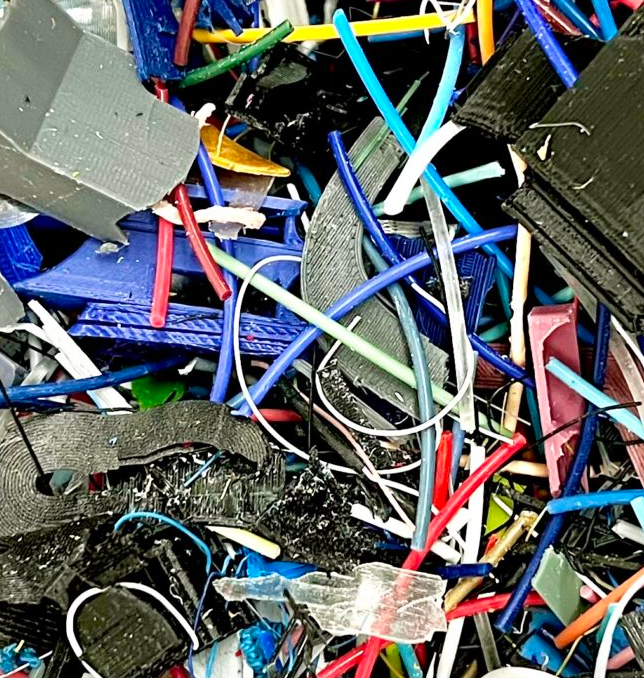
\includegraphics[width=3cm]{img/Reste}};
            \end{tikzpicture}
        }%
        \raisebox{1.5cm}{\LARGE$\longrightarrow$}%
        \subfloat[\centering Granulat]{
            \centering
            \begin{tikzpicture}
                \clip (0,0) circle (1.5cm) node {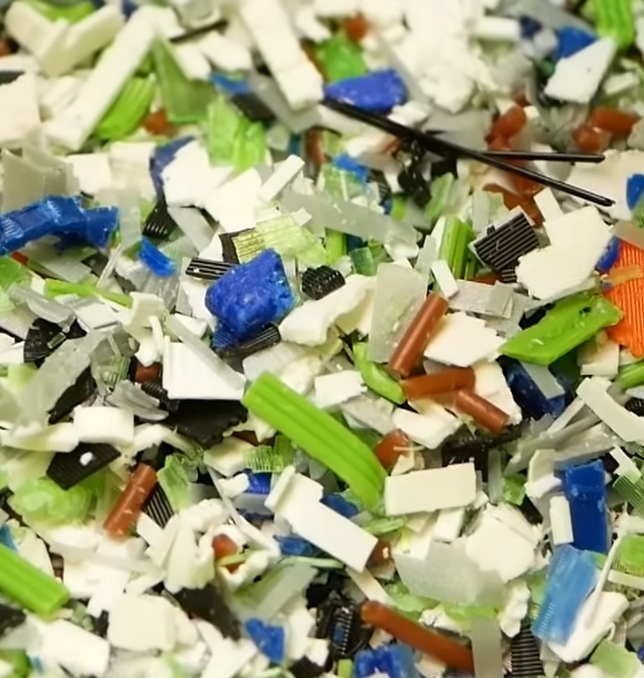
\includegraphics[width=3cm]{img/Geschreddert}};
            \end{tikzpicture}
        }%
        \raisebox{1.5cm}{\LARGE$\longrightarrow$}%
        \subfloat[\centering Filament]{
            \centering
            \begin{tikzpicture}
                \clip (0,0) circle (1.5cm) node {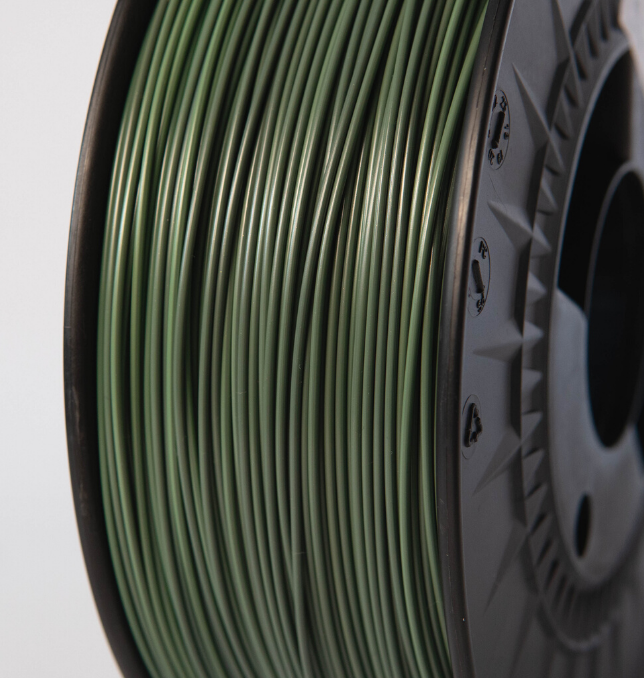
\includegraphics[width=3cm]{img/Filament}};
            \end{tikzpicture}
        }%
    \end{figure}


    \newpage
    \subsection{Kunststoffe und ihre Eigenschaften}
    Wie bereits erwähnt, kann man so gut wie alle Kunststoffe zum 3D-Druck verwenden.
    Damit ein Kunststoff jedoch für den FDM-Druck geeignet ist, müssen bestimmte Dinge beachtet werden.

    \begin{itemize}
        \item Schmelztemperatur
        \item Wärmeformbeständigkeit
        \item Schmelzviskosität
        \item Schrumpfverhalten
        \item Abrasivität
    \end{itemize}
    Die Schmelztemperatur darf nicht zu hoch sein, da der Kunststoff sonst zu langsam abkühlt und sich dadurch verzieht.
    Sie darf aber auch nicht zu niedrig sein, da der Kunststoff bei Wärme nicht formbeständig genug ist und sich dadurch auch ungewollt verformt.
    Ungewolltes Verformen aufgrund von Wärme ist das sogenannte Warping. \\
    Ist die Viskosität des Kunststoffs zu hoch, kann er nicht mehr durch die Düse gepresst werden und verstopft diese. \\
    Ist die Viskosität zu niedrig, kann der Kunststoff nicht mehr in Form gehalten werden und verläuft. \\
    Wenn der Kunststoff nach dem Abkühlen zu sehr schrumpft, kann sich das Druckobjekt vom Druckbett lösen und die Genauigkeit der Druckergebnisse ist nicht mehr gewährleistet. \\
    Ist der Kunststoff oder ein Zusatzmaterial im Filament abrasiv, dann reibt es die Düse ab und beschädigt diese. \\
    Um abrasives Material zu drucken, gibt es spezielle Düsen, die z.B. aus gehärtetem Stahl bestehen oder einen Edelstein an der Spitze haben. \\

    \begin{figure}[H]
        \centering
        \subfloat[\centering Stahl Düse]{{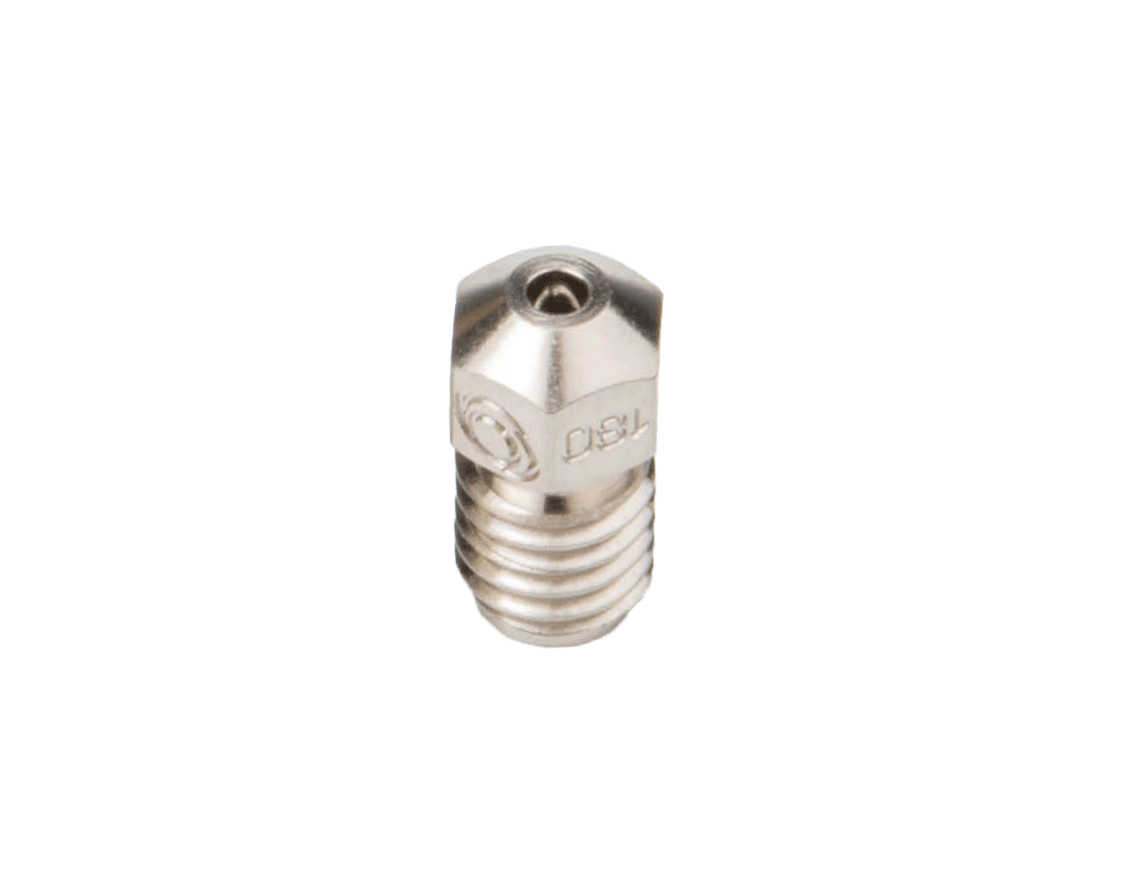
\includegraphics[width=4cm]{img/Steel_Nozzle}}}%
        \qquad
        \subfloat[\centering Rubin Spitze]{{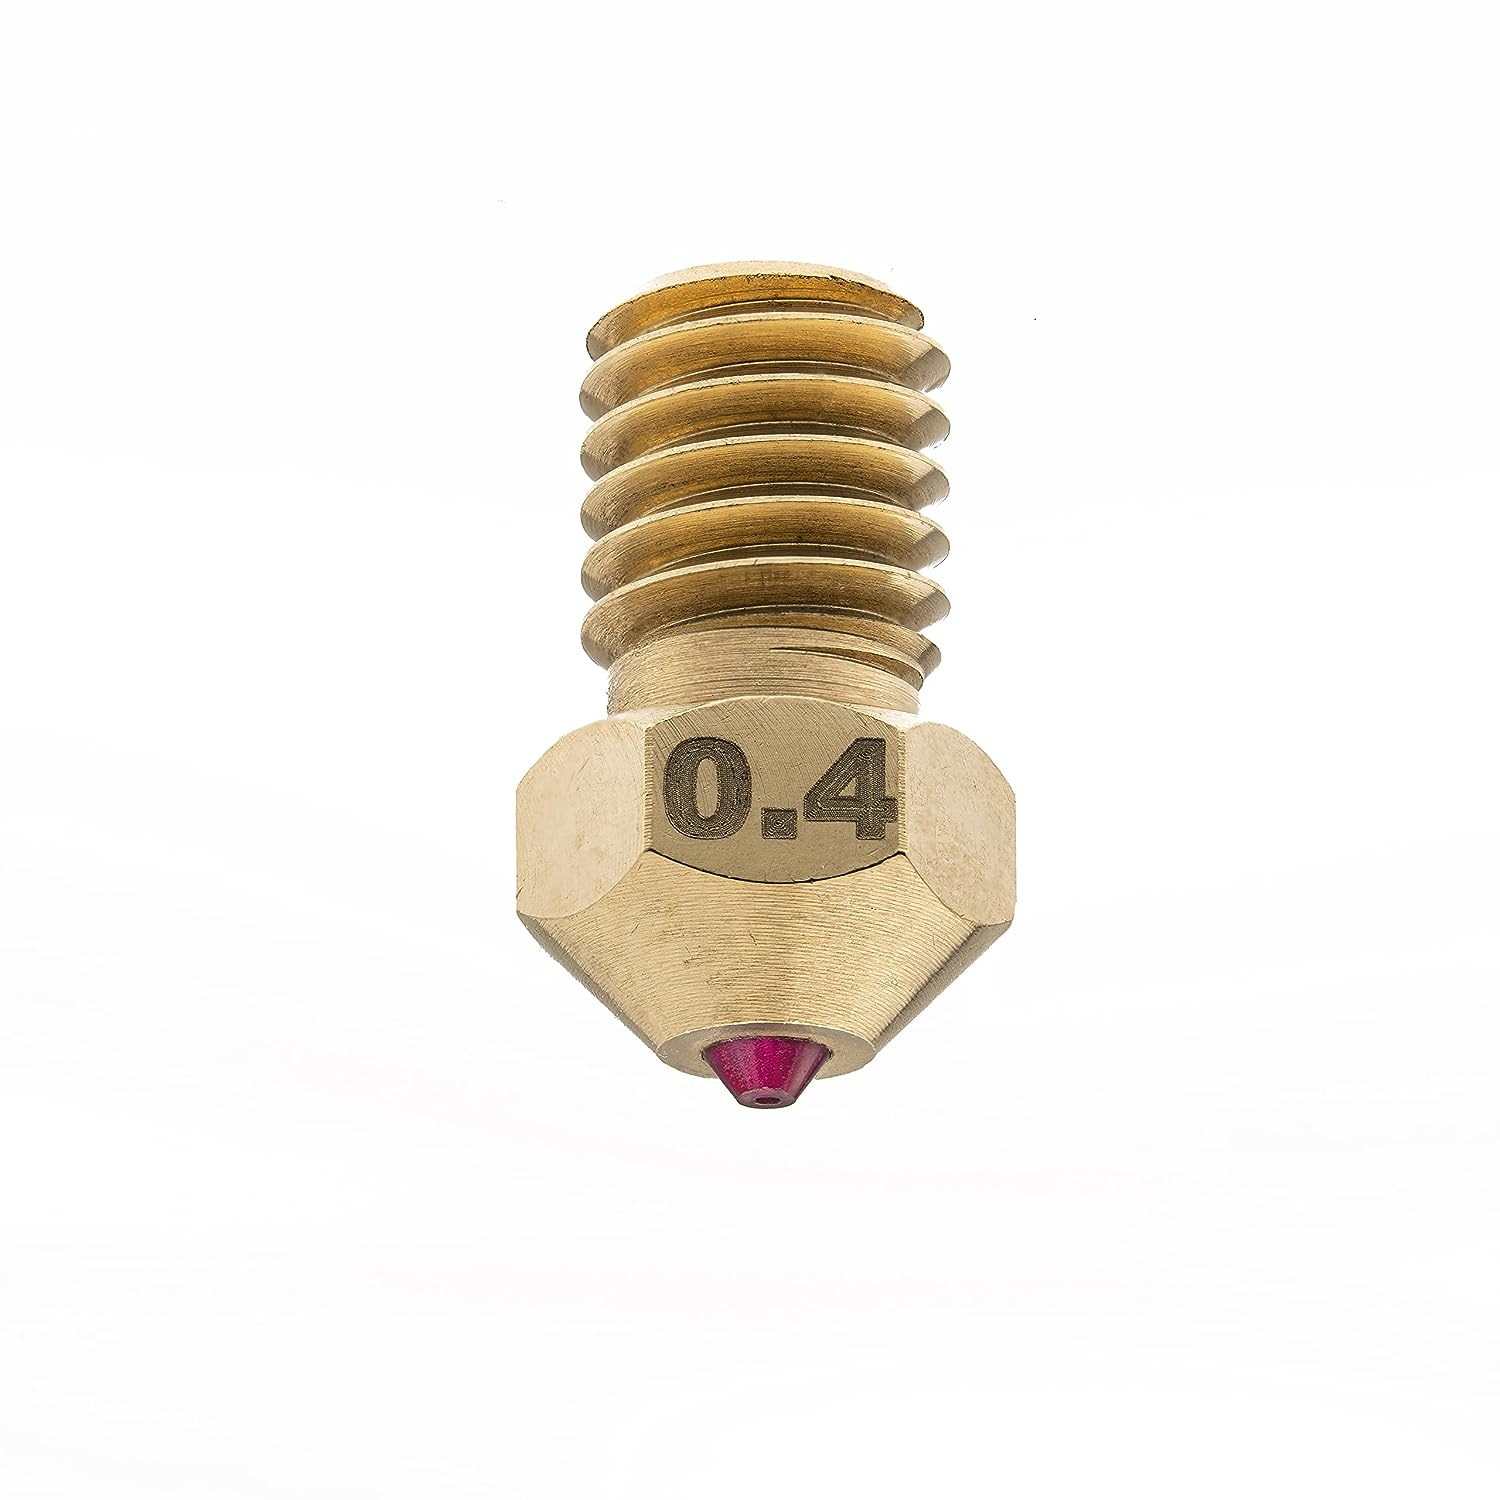
\includegraphics[width=4cm]{img/Ruby_nozzle}}}%
    \end{figure}

    \newpage
    \subsection{Filamentarten}
    Zu den gängigsten Filamentarten gehören PLA, PETG, ABS / ASA, TPU, Nylon und PC.
    PLA ist das am weitesten verbreitete Filament, das aus Mais hergestellt wird und biologisch abbaubar ist.
    Es ist einfach zu drucken, da es eine geringe Schmelztemperatur hat und kann daher sehr schnell gedruckt werden, es ist auch nicht abrasiv und muss auch nicht in einem beheizten Druckraum gedruckt werden.
    Es ist jedoch nicht sehr stabil, recht spröde und wird bereits bei 60°C weich.
    Zudem ist es absolut nicht chemisch beständig und zersetzt sich bei UV-Strahlung.
    Daher eignet es sich für Dekorationen, oder für Prototypen, die nicht lange halten müssen oder für Teile, die nicht mechanisch belastet werden.
    Etwas beständiger ist PETG. Es ist etwas flexibler als PLA und hat eine höhere Schmelztemperatur.
    Es ist zudem stabiler und chemisch beständiger als PLA, jedoch nicht UV-beständig.
    Es eignet sich für mechanische Teile mit geringer Belastung oder Möbel im Innenbereich.
    ABS ist noch stabiler und steifer als PETG, es kann auch höheren Temperaturen standhalten, jedoch muss es in einem beheizten Druckraum gedruckt werden, da es sonst zu Warping kommt.
    Abgesehen vom 3D-Druck wird es im Spritzguss oft verwendet z.B. Legosteine, Playmobil oder auch Auto- und Motorradteile.
    ABS hat den Nachteil oder auch Vorteil, dass es durch Aceton aufgelöst werden kann, was man sich beim 3D-Druck zunutze machen kann, um Teile zu verkleben oder zu glätten.
    ASA ist eine Variante von ABS, die UV-beständig ist und sich daher für den Außenbereich eignet.
    TPU ist ein flexibles Filament, das sich für Dichtungen, Stoßdämpfer oder Schutzhüllen eignet.
    TPU ist daher aber schwerer zu drucken, da das Zahnrad des Extruders das Filament schlechter greifen kann.

    Nylon und Polycarbonat sind sehr stabile Filamente, die sich für mechanische Teile eignen, die hohen Belastungen ausgesetzt sind.
    Sie sind aber sehr schwer zu drucken, da sie eine hohe Schmelztemperatur haben und sehr abrasiv sind.

    Es gibt natürlich noch viele weitere Filamente, z.B. Holzfilament für Holzoptik oder PVA für Stützstrukturen, die sich in Wasser auflösen, aber sie sind nicht so weit verbreitet. \\

    \begin{table}[H]
        \begin{tabular}{|l|c|c|c|c|c|c|}
            \hline
            \textbf{Filament} & \textbf{PLA} & \textbf{PETG} & \textbf{ASA} & \textbf{TPU} & \textbf{Nylon} & \textbf{PC} \\
            \hline
            \textbf{Drucktemperatur} & 190-230°C & 230-260°C & 225-255°C & 210-230°C & 220-270°C & 260-310°C \\
            \hline
            \textbf{Druckbett} & 60°C & 80°C & 90-110°C & 60°C & 70-90°C & 80-120°C \\
            \hline
            \textbf{Preis pro kg} & 20-30\officialeuro & 20-30\officialeuro & 20-30\officialeuro & 20-30\officialeuro & 40-60€ & 40-60\officialeuro \\
            \hline
            \textbf{Stabilität} & Niedrig & Mittel & Hoch & Mittel & Hoch & Hoch \\
            \hline
            \textbf{Steifheit} & Hoch & Mittel & Hoch & Niedrig & Mittel & Hoch \\
            \hline
            \textbf{UV-Beständigkeit} & Nein & Nein & Ja & Nein & Nein & Ja \\
            \hline
            \textbf{Chemische Beständigkeit} & Niedrig & Mittel & Mittel & Mittel & Mittel & Hoch \\
            \hline
        \end{tabular}
    \end{table}

    \newpage

    \section{PLA herstellung}

    Biologisch Abbaubar.
    Hergestellt aus Zucker (Fermentation).
    aus Maisstärke, weizen, Stroh, Hirse
    Zerfällt zy Wasser und CO2 durch Mikroorganismen.

    170-230°C Verarbeitungstemperatur

    Biokompatibilität, biologische Abbaubarkeit, Glanz und Transparent, antibakteriell, öl-wasserbeständig
    Verpackungsmaterial, Vliesstoffe, Kleidung, medizinische Anwendungen (Fäden, Implantate, OP-Material),

    lactic acid (Milchsäure)
    1881 aus fermentierter Milch  oder aus Zucker durch Bakterien

    D-laic acid aus Tiermuskeln

    Fermentation:
    3-5 Tage, niedriger pH (5), wenig Sauerstoff, 40°C
    Wird mit der Zeit giftig desto mehr Milchsäure sich bildet.
    > Ammoniak und Natriumhydroxid reinigen

    \begin{figure}[H]
        \centering
        \subfloat[\centering L-lactic acid]{\chemfig{[:-30]HO-(<[:210]H_{3}C)(<:[:-40]CH_{3})-[:30](=[2]O)(-[:-30]OH)}}%
        \qquad
        \subfloat[\centering D-lactic acid]{\chemfig{[:-30]HO-(<[:210]H_{3}C)(<:[:-40]H)-[:30](=[2]O)(-[:-30]OH)}}%
    \end{figure}

    PLA-Polymerisation:
    Lacitc acid ist chiral = Asymmetrisches Molekül
    D- und L-Form
    P-L-LA: Entzündend, da langsamer Abbau im Körper
    P-D-LA: schneller Abbau im Körper
    P-D-L-LA: Bestes von beiden

    2-Schritt Synthese
    1. Dehydratisierungkondensation von Hydroxylgruppen und Carboxylgruppen in äquimolaren Konzentrationen
    => niedermolekulares PLA (Polymilchsäure)

    2. Kopplungsmittel und Veresterungsbeschleuniger hinzufügen
    => hochmolekulares PLA (Längere Ketten)

    -> Für bessere Reinheit Triphosgen
        -> Teurer und gefährlich

    Azeotropische Dehydratisierungskondensation
    1. Milchsäure destillieren bei 130°C und niedrigem Druck für 2-3h
    2. Katalysator und Diphenylether zur Reaktion hinzufügen.
    3. In Molekularsieb geben und für 30-40h bei 130°C in Behälter zurückführen.
    4. Polymer zur reinigung abtrennen, gelöst oder ausgefällt. Dannach höherer Siedepunkt des Lösungsmittel weil weniger Wasser -> schnellere Polymerisation

    Zinnverbindungen als Katalysator

    \begin{figure}[H]
        \centering
        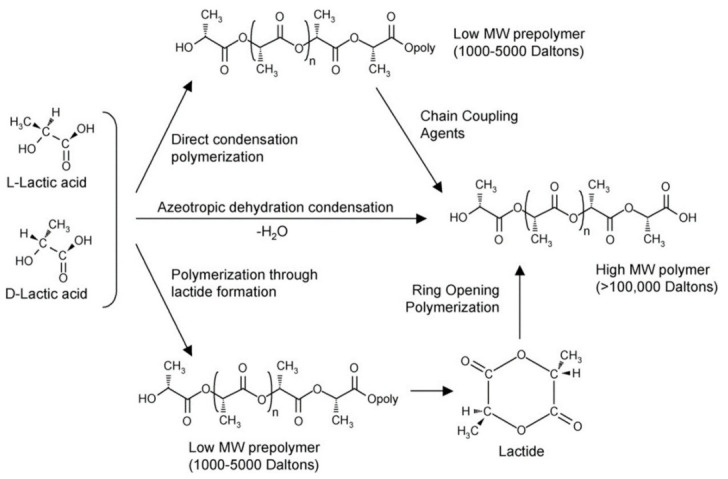
\includegraphics{img/PLA_synthese}
    \end{figure}

    ---

    \subsection{Introduction}
    PLA bzw. Polymilchsäure ist ein Biopolymer, das aus erneuerbaren Ressourcen wie Weizen, Stroh, Mais und Hirse gewonnen wird.
    Es ist umweltfreundlich, da es von Mikroben zu Wasser und Kohlendioxid abgebaut werden kann.
    Zudem liegt die Verarbeitungstemperatur zwischen 170 und 230°C, wodurch es für Extrusions-, Spinn-, biaxiale Streck- und Spritzblasformverfahren geeignet ist.
    PLA hat auch eine gute Biokompatibilität, Bioabbaubarkeit, Glanz und Transparenz sowie antibakterielle, flammhemmende, öl- und wasserabweisende Eigenschaften.
    Dadurch kann es in vielen Bereichen eingesetzt werden, z.B. als Verpackungsmaterialien, Vliesstoffe, Kleidung und medizinische Anwendungen (Fäden, Implantate, OP-Material).

    \subsection{Milchsäure}
    Milchsäure wurde erstmals aus fermentierter Milch extrahiert, und ist ein wichtiger Bestandteil des glycolytischen Energiekreislaufs von Organismen.
    Das Molekül der Milchsäure enthält ein asymmetrisches Kohlenstoffatom auch chirales Zentrum genannt, das optisch aktiv ist.
    Ist ein Molekül optisch aktiv, bedeutet das, dass es zwei optische Isomere gibt, die sich zueinander verhalten wie Bild und Spiegelbild.
    Das bedeutet, es gibt zwei optische Isomere, L-Milchsäure und D-Milchsäure.
    Einfach gesagt, dreht L-Milchsäure polarisiertes Licht nach links und D-Milchsäure nach rechts.
    L-Milchsäure wird aus Tiermuskeln gewonnen, während D-Milchsäure durch Fermentation gewonnen wird.



    Als einfachste Hydroxysäure enthält das Molekül ein asymmetrisches Kohlenstoffatom, das optisch aktiv ist, so dass es zwei optische Isomere, L-Milchsäure und D-Milchsäure, gibt, wie in Abbildung 1 gezeigt [21,22].
    Milchsäure, die aus Tiermuskeln gewonnen wird, ist dextrorotatorische Milchsäure, während die andere, durch Fermentation gewonnene Milchsäure levogyre Milchsäure ist.
    Anfangs wurde kommerzielle Milchsäure hauptsächlich durch die Fermentation von Zuckern durch Bakterien gewonnen [23].
    Für die Milchsäurefermentation verwendete Zucker umfassen Stärke, Glukose, Laktose und Maltose, die durch Mais und Kartoffeln produziert werden.
    Die Fermentation wird typischerweise 3-5 Tage lang bei niedrigem pH-Wert (ca.\ 5,0) und niedrigem Sauerstoffgehalt bei einer Temperatur von etwa 40 °C durchgeführt [24].
    Allerdings erzeugt dieses Verfahren einen gewissen Grad an Toxizität, da sich die Konzentration der fermentierten Milchsäure erhöht und die Reaktion weitergeht.
    Um hochreine Milchsäure zu erhalten und die Ausbeuteeffizienz der Milchsäure zu verbessern, stellt auch die Reinigung ein großes Problem dar [25].
    Anfangs war die typische Reinigungsmethode, Kalziumhydroxid oder Kalziumkarbonat zur Neutralisation der Säure in den Gärungsbrüden hinzuzufügen.
    Das resultierende Kalziumlaktat konnte verdampft, kristallisiert und angesäuert werden, um weitere Rohmilchsäure und unlösliche Kalziumsulfat (Gips) zu erhalten.
    Milchsäure, die in Lebensmitteln oder Medikamenten verwendet wird, muss oft weiter aufgereinigt werden, um einen höheren Milchsäuregrad zu erhalten.
    Spätere Studien zeigten, dass sie dann mit recyceltem Ammoniak oder Natriumhydroxid neutralisiert werden kann.
    Anschließend wurden Ultrafiltration, Färbung und Elektrodialyse als neue Verfahren für die kostengünstige Produktion von Milchsäure entwickelt [26].

    Obwohl chemische Methoden in der Lage sind, die Großproduktion von Milchsäure kontinuierlich durchzuführen, und das resultierende Produkt von der US-Arzneimittelbehörde FDA zugelassen wurde, sind die Ausgangsstoffe im Allgemeinen giftig.
    Sie entsprechen nicht den Standards der grünen Chemie.
    Einige neuere Studien zeigten, dass durch Hinzufügen von Bakterien und substratabbauenden Enzymen zur gleichzeitigen Saccharifizierung und Fermentation Stärke oder cellulosische Biomasse in Zucker umgewandelt und gleichzeitig in Milchsäure umgewandelt werden kann; dieser Prozess kann die oben genannten traditionellen Fermentationsschritte ersetzen [28,29].
    Dieser Prozess reduziert Kosten und verbessert die Effizienz.

    \subsection{Polymilchsäure}

    Da Milchsäure ein chirales Molekül mit D- und L-Isomeren ist, bilden sich drei Formen von Polymilchsäure: Poly-L-Milchsäure (PLLA), Poly-D-Milchsäure (PDLA) und Poly-D,L-Milchsäure (PDLLA). In Bezug auf die optische Aktivität gibt es zwei Zusammensetzungen – L- und D-Enantiomere –, so dass Polymilchsäure in drei Formen (α, β und γ) kristallisiert werden kann [30,31,32].
    1932 synthetisierte Carothers (DuPont) Polymilchsäureprodukte mit niedrigem Molekulargewicht.
    Aufgrund der hohen Herstellungskosten und der schlechten Produktstabilität galt diese Synthese jedoch nicht als Erfolg [33].
    1954 produzierte DuPont eine Polymilchsäure mit höherem Molekulargewicht und meldete ein Patent an, um in den Handel einzusteigen.
    Die Forschung an Polymeren erregte in der Gesellschaft große Aufmerksamkeit.
    Mit den Fortschritten in der Medizin und im öffentlichen Gesundheitswesen begann Polymilchsäure in den 1960er Jahren für chirurgische Nähte und Knochenimplantate verwendet zu werden.
    Heutzutage wurde PLA-Harz von der FDA und den europäischen Aufsichtsbehörden für den Einsatz in Lebensmittel- und Arzneistofffreisetzungssystemen zugelassen [12,34].
    Dies hat die Menschen auch dazu gebracht zu erkennen, dass PLLA zwar einige Vorteile hat, aber auch einige Nachteile.
    Zum Beispiel kann es aufgrund seiner hohen Kristallinität und langsamen Abbaurate eine Entzündungsreaktion im Körper auslösen.
    Glücklicherweise baut sich D-Milchsäure schneller ab.
    Wenn L-Milchsäure und D,L-Milchsäure-Monomere verwendet werden, um PLLA zu synthetisieren, werden die oben genannten Probleme vermieden [35,36].

    Drei Methoden zur Synthese des Polymers PLA (Mw > 10.000) wurden berichtet: (a) direkte Kondensationspolymerisation; (b) azeotrope Dehydratisierungskondensation und (c) Lactid-Ringöffnungspolymerisation, wie in Abbildung 2 dargestellt.

    Obwohl die Kosten der Kondensationspolymerisationsmethode niedrig sind, kann sie nicht direkt Polymer-PLA synthetisieren.
    Vielmehr entspricht ein Teil der Kosten dem Kupplungsmittel und Beschleuniger, die im Syntheseprozess verwendet werden.
    Der Syntheseschritt ist in zwei Schritte unterteilt [37,38,39].
    Der erste Schritt ist die Dehydratisierungskondensation von Hydroxyl- und Carboxygruppen in äquimolaren Konzentrationen zur Herstellung von niedermolekularer Polymilchsäure.
    Anschließend müssen Kupplungsmittel und Veresterungsadjuvantien hinzugefügt werden.
    Ihre Zugabe kann die PLA modifizieren und die Kette verstärken helfen.
    Im nachfolgenden Produktionsprozess konnte jedoch aufgrund der effizienten Wasserentfernung der Siedepunkt des Lösungsmittels erhöht und damit die Polymerisationsrate erhöht werden.
    Nach dem Test einer Vielzahl von Katalysatoren stellte sich heraus, dass Zinnverbindungen eine höhere katalytische Effizienz aufweisen.
    Darüber hinaus behindern die Verunreinigungen die Synthese in gewissem Umfang.
    In der anschließenden Industrieforschung wurde gezeigt, dass es möglich ist, den Katalysator zu einem großen Teil zu entfernen, ohne das Polymer zu zersetzen.
    Die Toxizität und Nichtabbaubarkeit des restlichen Katalysators kann jedoch irreparable Schäden am menschlichen Körper verursachen, sodass er nicht im medizinischen Bereich angewendet werden kann.

    \subsection{Ringöffnungspolymerisation}

    Die Ringöffnungspolymerisation von Lactid ist eine der Methoden für die industrielle Produktion von hochmolekularem PLA. Lactid hat drei Stereokonfigurationen - l-Lactid, Mesolactid und d-Lactid - wie in Abbildung 3 gezeigt [42].
    Als zyklisches Dimer kann es durch lösungsmittelfreie Dehydratisierung unter milden Bedingungen gebildet werden.
    Kommerziell realisierbare Methoden zur Gewinnung und Reinigung von Lactid umfassen Schritte wie die Kondensation von Milchsäure bei 115-179 °C, die Entfernung des Kondenswassers und die Entfernung der Mesomilchsäure und des niedermolekularen Polymers durch Umkristallisation, um reines l- oder d,l-Lactid mit hohem Molekulargewicht zu erhalten [9,43,44].
    Das industrielle Herstellungsverfahren für Lactid ist das gleiche wie das oben erwähnte Schema, aber in unterschiedlichen Reaktoren, wobei Vorpolymere mit niedrigem Molekulargewicht erzeugt werden, und die endgültige Reinigungsmethode ist eine andere.
    Zum Beispiel verwendet Cargill Inc.
    ein Verfahren mit vermindertem Druck-Rückfluss, um Restwasser, Milchsäure, Oligomere und teilweises Lactid zu entfernen [45].
    Nemphos änderte den Reinigungsschritt und verwendete einen Mehrstufen-Schmelzrekristallisator, um LA und niedermolekulares Polymer zu entfernen.
    Bhatia und Kollegen verwendeten Inertgas, um Lactid zu entfernen, umzukristallisieren und zu reinigen.
    Andere Methoden umfassen die Verwendung von Lactid zur Gasphasen-Umkristallisation, um die Ausbeute zu erhöhen, und schwach alkalische Wasser-/Lösungsmittelsysteme, um Lactid zu extrahieren.
    Bei dem oben beschriebenen Verfahren wird nach der Entfernung von Verunreinigungen im Allgemeinen hochreines Lactid erhalten.

    Nachdem hochreines Lactid erhalten wurde, kann die Ringöffnungspolymerisation von Lactid je nach Katalysator einem von drei Mechanismen folgen: Kationisch, anionisch und Koordinations-/Insertionsmechanismus.
    Kationische Initiatoren können im Allgemeinen in protische Säuren, Lewis-Säuren und alkylierende bzw.
    acylierende Reagenzien unterteilt werden.
    Kricheldorf und seine Kollegen fanden heraus, dass Triflsäure und Methyltriflat unter vielen kationischen Initiatoren die Polymerisation von Lactid wirksam induzieren können.
    Die Wahl verschiedener Anion-Induktoren bewirkt eine Deprotonierung, was zu einer inkonsistenten Polymerisation und Racemisierung führt, was wiederum zu Polymeren mit unterschiedlichen Molekulargewichten führt [46].
    In Anbetracht, dass Metallionen Toxizitätsprobleme verursachen können, wird die Verwendung von Butyllithium oder Kronenether-Initiatoren nicht empfohlen.
    Die Verwendung von primären Alkoxiden, 6-Valerolacton oder Polyethylenglykol kann eindeutig definierte Polymere erzeugen.
    Die beiden oben genannten Methoden haben eine hohe Reaktivität und neigen gewöhnlich während des Lösungsmittelreaktionsprozesses zu Racemisierung und Transesterifizierung, was zu Verunreinigungen führt.
    Die Verwendung von Metallcarboxylaten, -oxiden und -alkoxiden mit geringerer Aktivität zur Herstellung von Polylactid mit geringer Toxizität und wenigen Verunreinigungen wurde in kommerziellen Produktionsanwendungen ausführlich untersucht.
    Studien haben gezeigt, dass die Verwendung von Zinn (II) und Zink bei der Synthese von hochmolekularer Polymilchsäure zu weniger Verunreinigungen führt, was zu der reinsten Polymilchsäure führt.
    Zum Beispiel hat Zinn(II)-di-2-ethylhexanoat eine hohe katalytische Aktivität und geringe Toxizität.
    Es wurde von der FDA zugelassen und ist ein äußerst geeigneter Induktor.
    Neben Zinnverbindungen sind Aluminiumalkoxide und Seltenerdverbindungen andere Katalysatorsysteme, die über Koordinations-/Insertionsmechanismen ablaufen.
    Die Forschung ergab, dass die Polymerisationsrate von Seltenerdverbindungen immer noch viel höher ist als die von Aluminiumalkoxiden.

    Darüber hinaus ist laut Forschung die enzymatische Polymerisation umweltfreundlicher als chemische Synthesemethoden.
    Enzymatische Reaktionen erfordern ein mildes Umfeld, und Enzyme sind effizient, kostengünstig und hochspezifisch.
    Chemische Reaktionen erfordern ein einzelnes Reaktant, um Nebenreaktionen zu vermeiden.
    Es sind jedoch nicht viele Referenzen für diese Methode verfügbar [47].


    ---
    Die Esterbindungen des Polymerrückgrats werden durch Hydrolyse ohne zusätzliche Operationen gespalten, und die Abbauprodukte sind ungiftig und vermeiden einen Teil der Immunantwort, was es zu einem idealen Kandidaten für biomedizinische Anwendungen macht.

    ---


    \section{FDM-Druck}
    Wie man mit Filamenten druckt.


\end{document}







